\documentclass[xetex,mathsans,sans]{beamer}
\usetheme{Boadilla}
\usecolortheme{orchid}
\usepackage{fontspec}
\setsansfont{Basis Grotesque}


\title[NuCypher KMS]{NuCypher KMS: Decentralized Key-Management System}
\author[Michael]{Michael Egorov, CTO}
\date[29 Nov 2017]{SF Cryptocurrency Devs, 29 Nov 2017}

\begin{document}
    \begin{frame}
        \titlepage
        \begin{figure}
            \centering
            
\includegraphics[width=5cm]{pdf/nucypher_logo.pdf}
        \end{figure}
    \end{frame}

    \begin{frame}
        \frametitle{Why}
        \framesubtitle{Encrypted file sharing}
        \begin{figure}
            \centering
            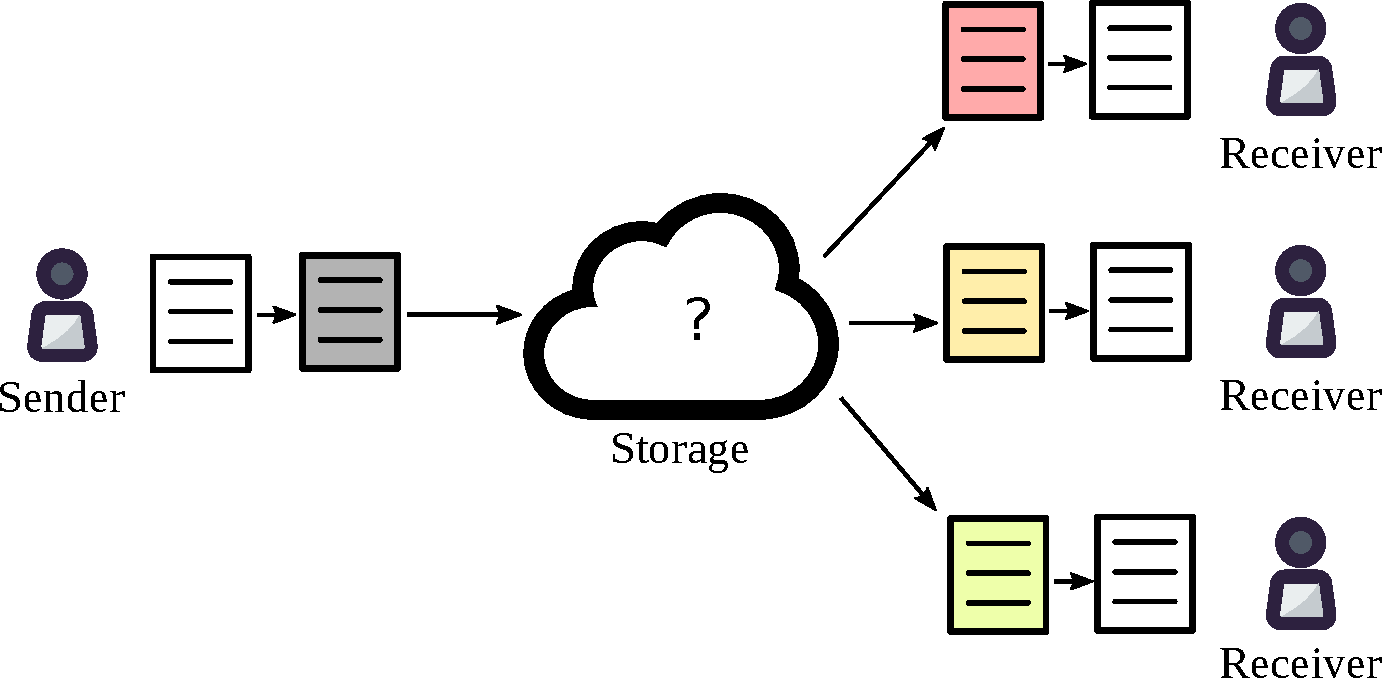
\includegraphics[height=5.5cm]{pdf/file-sharing.pdf}
        \end{figure}
    \end{frame}

    \begin{frame}
        \frametitle{Why}
        \framesubtitle{Encrypted multi-user chats}
        \begin{figure}
            \centering
            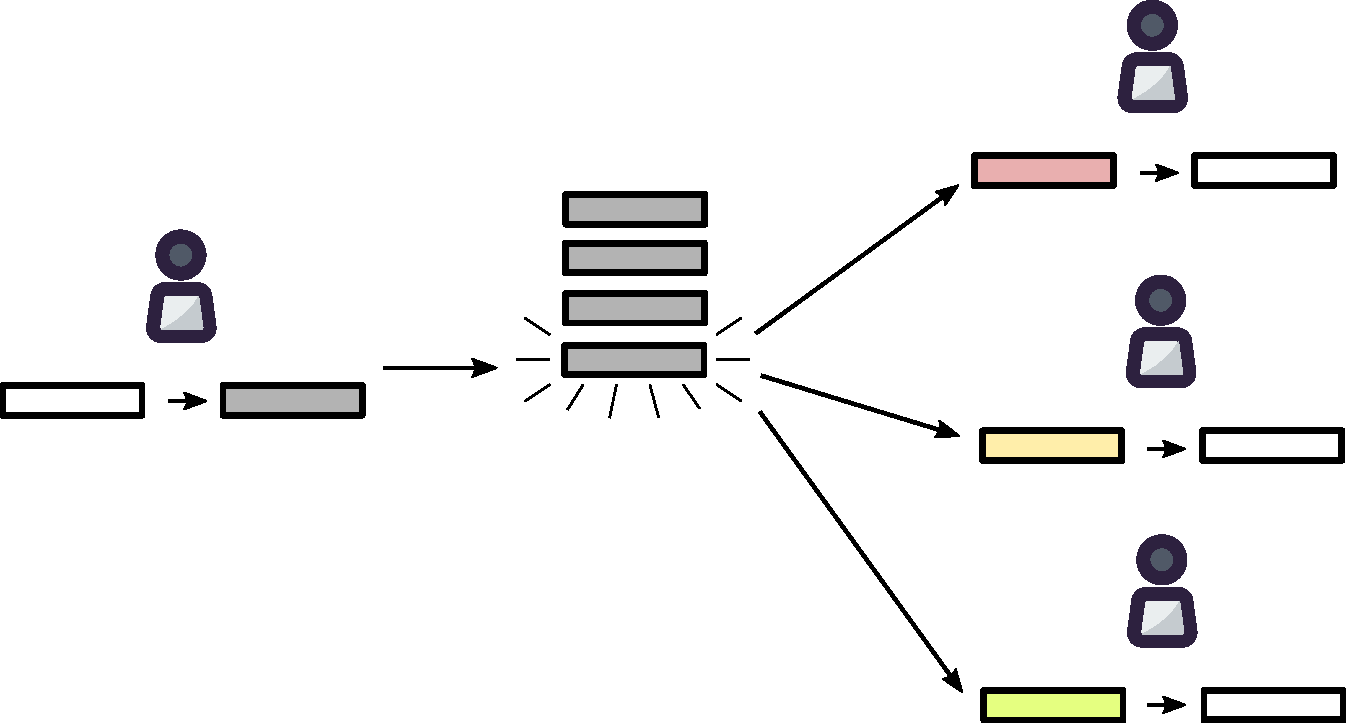
\includegraphics[height=5.5cm]{pdf/chats.pdf}
        \end{figure}
    \end{frame}

    \begin{frame}
        \frametitle{Why}
        \framesubtitle{Decentralized Netflix}
        \begin{figure}
            \centering
            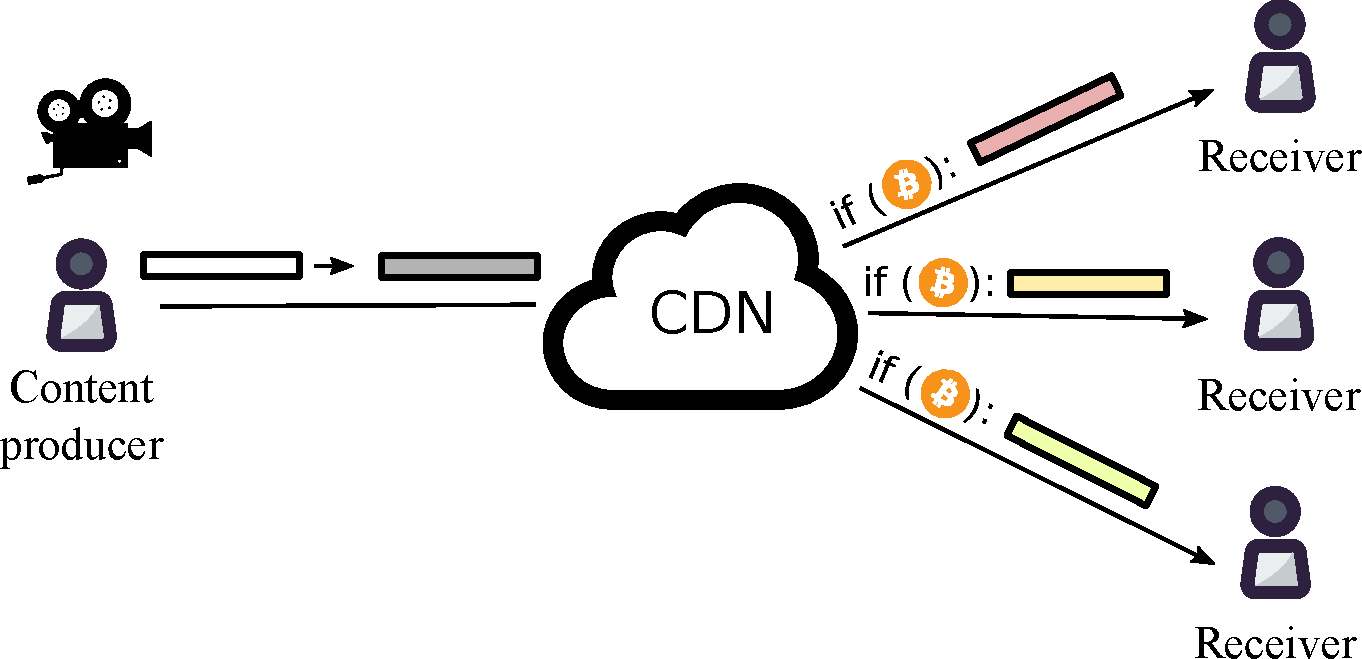
\includegraphics[height=5.5cm]{pdf/streams.pdf}
        \end{figure}
    \end{frame}

    \begin{frame}
        \frametitle{Central server + TLS}
        \framesubtitle{Data vulnerable to hackers, state actors etc}
        \begin{figure}
            \centering
            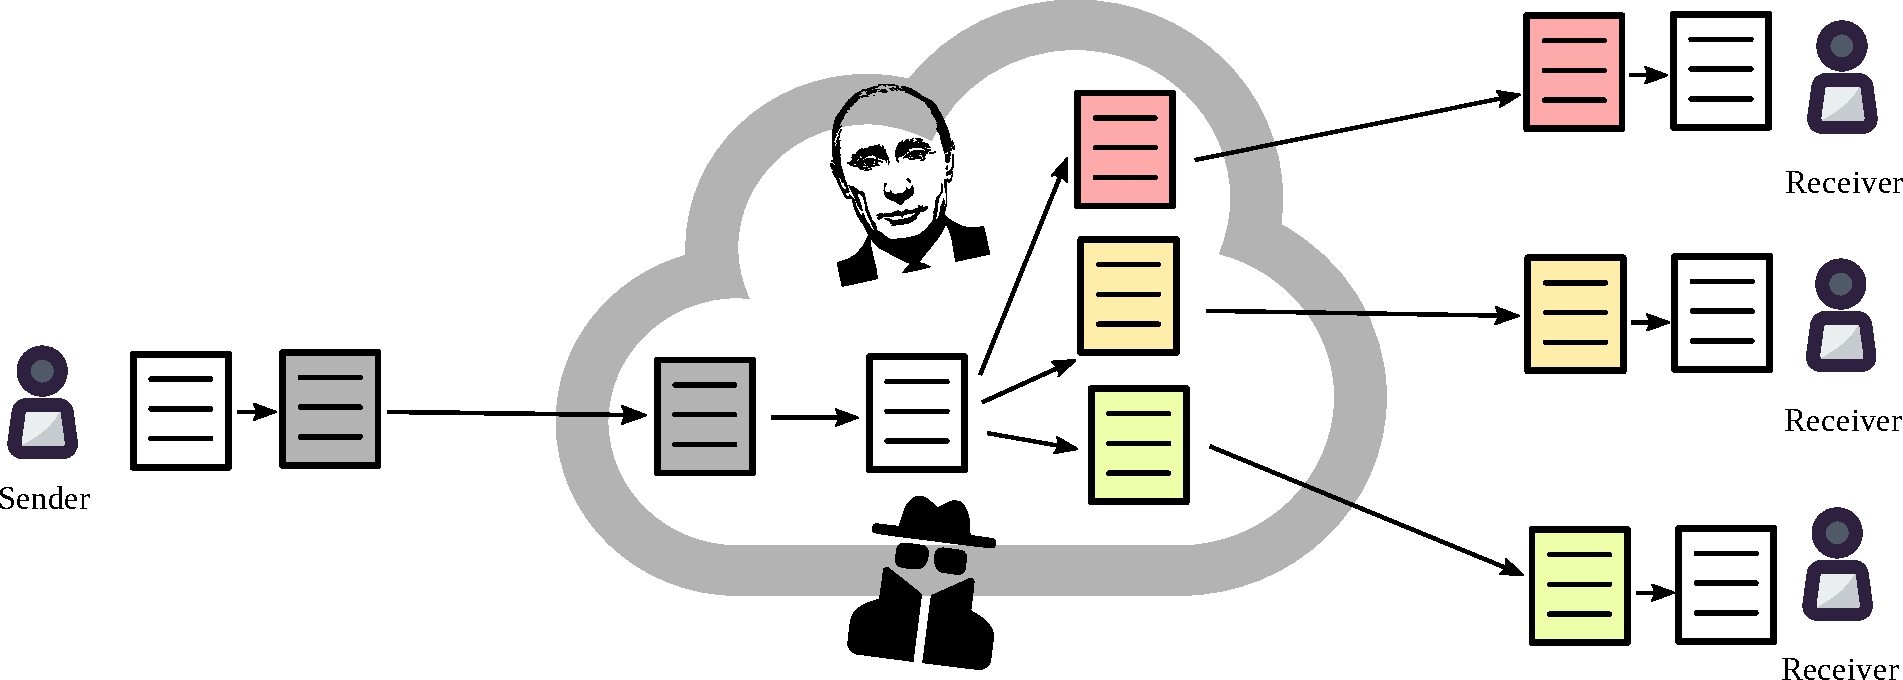
\includegraphics[width=11cm]{pdf/file-sharing-tls.pdf}
        \end{figure}
    \end{frame}

    \begin{frame}
        \frametitle{Solution}
        \framesubtitle{Proxy re-encryption + decentralization}
    \end{frame}

    \begin{frame}
        \frametitle{What is proxy re-encryption (PRE)}
    \end{frame}

    \begin{frame}
        \frametitle{PRE demo}
    \end{frame}

    \begin{frame}
        \frametitle{Centralized KMS using PRE}
        \framesubtitle{Still too much power}
    \end{frame}

    \begin{frame}
        \frametitle{Threshold split-key re-encryption (Umbral)}
    \end{frame}

    \begin{frame}
        \frametitle{Decentralized KMS network}
    \end{frame}

    \begin{frame}
        \frametitle{KMS token}
    \end{frame}

    \begin{frame}
        \frametitle{KMS token}
        \framesubtitle{Mining}
    \end{frame}

    \begin{frame}
        \frametitle{Investors}
    \end{frame}

    \begin{frame}
        \frametitle{Early users}
    \end{frame}

    \begin{frame}
        \frametitle{Team}
    \end{frame}

    \begin{frame}
        \frametitle{How to contribute, learn}
    \end{frame}
\end{document}

